% Converted to MDPI Sensors format (MDPI LaTeX class, 25 March 2023).
\documentclass[sensors,article,submit,pdftex,moreauthors]{Definitions/mdpi}

%=================================================================
% MDPI internal commands - do not modify
\firstpage{1}
\pubvolume{1}
\issuenum{1}
\articlenumber{0}
\pubyear{2026}
\copyrightyear{2026}
\datereceived{ }
\daterevised{ }
\dateaccepted{ }
\datepublished{ }
\hreflink{https://doi.org/}

%=================================================================
% Packages required by this manuscript. The MDPI class already loads
% amsmath, amssymb, graphicx, booktabs, tikz, hyperref, caption, etc.
\usepackage{pgfplots}
\pgfplotsset{compat=1.17}
\usetikzlibrary{arrows.meta,positioning,calc,fit}
\usepackage{subcaption}
\usepackage{siunitx}

% Author ORCID identifiers
\newcommand{\orcidauthorA}{0009-0006-0447-0482} % Qinmin Wang
\newcommand{\orcidauthorD}{0009-0007-4278-771X} % Hongyuan Wang
\newcommand{\orcidauthorE}{0009-0006-0345-654X} % Liwei Tian

%=================================================================
\Title{Joint Detection and Azimuth Estimation of UAVs Using MEMS Microphone Arrays and Multi-Task Deep Learning: From Simulation to Real-World Recordings}

\TitleCitation{Joint Detection and Azimuth Estimation of UAVs Using MEMS Microphone Arrays and Multi-Task Deep Learning: From Simulation to Real-World Recordings}

% Authors (order: 1 Qinmin Wang, 2 Zixin Wang, 3 Zhenzhen Hu, 4 Hongyuan Wang, 5 Liwei Tian*)
\Author{Qinmin Wang $^{1}$\orcidA{}, Zixin Wang $^{2}$, Zhenzhen Hu $^{3}$, Hongyuan Wang $^{1}$\orcidD{} and Liwei Tian $^{1,*}$\orcidE{}}

\AuthorNames{Qinmin Wang, Zixin Wang, Zhenzhen Hu, Hongyuan Wang and Liwei Tian}
\AuthorCitation{Wang, Q.; Wang, Z.; Hu, Z.; Wang, H.; Tian, L.}

\address{%
$^{1}$ \quad School of Computer and Artificial Intelligence, Guangdong University of Science and Technology, Dongguan 523083, China; wangqinmin@gdust.edu.cn (Q.W.); wanghongyuan@gdust.edu.cn (H.W.); tianliwei@gdust.edu.cn (L.T.)

$^{2}$ \quad College of Electronic and Communication Engineering, Tianjin Normal University, Tianjin 300387, China; 396514839@qq.com (Z.W.)

$^{3}$ \quad Chengdu University of Information Technology, Chengdu 610225, China; hzzuestc@163.com (Z.H.)}

\corres{Correspondence: tianliwei@gdust.edu.cn}

\abstract{The proliferation of UAVs in aerial photography, logistics, agriculture, and surveillance has created a demand for counter-UAV sensing that is passive, low-cost, and independent of illumination. Microphone arrays built from MEMS sensors meet these requirements, but most acoustic systems treat drone detection and direction-of-arrival (DOA) estimation as decoupled stages, preventing feature sharing and letting detection errors propagate into localization. This paper presents an end-to-end multi-task network that jointly detects a drone and regresses its azimuth from the raw multichannel waveforms of a six-element MEMS uniform linear array (ULA). A shared 1D-CNN backbone feeds a detection head and a DOA regression head, and an uncertainty-based dynamic weighting scheme balances the two losses during training. Monte Carlo simulations compare the proposed model with the classical TDOA baselines GCC-PHAT and SRP-PHAT: at $\mathrm{SNR}=-5\,\mathrm{dB}$ the joint model attains a detection probability of $0.99$ with no observed false alarms ($P_{\mathrm{fa}}=0.00$) and an azimuth MAE of $5.28^\circ\pm5.57^\circ$, reducing the GCC-PHAT and SRP-PHAT errors ($45.24^\circ$ and $44.91^\circ$) by roughly a factor of eight. Ablation confirms joint training is necessary: a detection-only branch learns no angle, whereas a localization-only branch yields no detection. Replacing the raw input with a geometry-aware GCC-PHAT frontend adapts the same backbone to the Fraunhofer IDMT recorded-drone corpus~\cite{idmt2025drone}; fine-tuning reduces the azimuth MAE from $45.6^\circ$ (zero-shot) to $18.1^\circ$---an optimistic in-sample estimate, not a generalization result.}

\keyword{direction-of-arrival estimation; MEMS microphone array; multi-task learning; UAV detection; Cram\'er--Rao bound}

% -------------------------------------------------------------------
% Clean typeset PDF: the MDPI class enables marginal line numbering in
% the 'submit' status; neutralise the switch so no line numbers are drawn.
\renewcommand{\linenumbers}{}
% -------------------------------------------------------------------
% The class-provided \bio command lays the author biography out in a fixed
% 13.86 cm pbox (Definitions/mdpi.cls), which is the width of the MDPI
% published text block but is wider than the 'submit' text width once the
% name column and the 1.1 cm gap are added -- it overflows the margin by
% ~77 pt. Redefine it with an adaptive width so the block fits this class's
% text width while keeping the same two-column name/text house layout.
\makeatletter
\renewcommand{\bio}[2]{\noindent\makebox[2.2cm][l]{#1}\noindent{\fontsize{9}{11.2}\selectfont \pbox[b]{\dimexpr\textwidth-2.2cm\relax}{#2}}\par\vspace{6pt}}
\makeatother
\begin{document}


\section{Introduction}
\label{sec:intro}
Unmanned aerial vehicles (UAVs) are now widely deployed for photography, delivery, agriculture, and infrastructure monitoring. Flights that violate airspace regulations, however, pose risks to public safety and privacy, and this has motivated sustained research on UAV detection and localization~\cite{taha2019drone}. Radio-frequency analysis, radar, and electro-optical sensors address this problem but are either active emitters, dependent on illumination, or too costly for wide-area deployment. Passive acoustic sensing with arrays of low-cost MEMS microphones is an attractive complement: it requires no emission, operates at night and in poor visibility, and has been demonstrated for UAV detection and tracking in several field studies~\cite{case2008uav,busset2015acoustic}. Practical MEMS arrays are, however, imperfect devices: element self-noise, channel-to-channel sensitivity mismatch, occasional channel failures, and geometry calibration errors all perturb the assumed array manifold~\cite{yan2023mems}, so a deployable estimator should tolerate an imperfect or only partially known array geometry. The geometry-aware frontend developed in Section~\ref{sec:geo} is a first step toward tolerating such non-ideal arrays, yet the simulation in this paper still assumes an ideal array manifold; explicit modeling of MEMS-specific impairments is left to future work.

A spinning rotor radiates a broadband, amplitude-modulated acoustic signature, and the inter-channel time delay of this signature across an array constrains the source direction. Classical pipelines estimate the direction of arrival (DOA) with generalized cross-correlation (GCC-PHAT)~\cite{knapp1976gcc}, steered-response power (SRP-PHAT)~\cite{dibiase2001srp}, or subspace methods such as MUSIC~\cite{schmidt1986music} and ESPRIT~\cite{roy1989esprit}, while a separate energy- or spectrum-based test decides whether a drone is present at all. This decoupling has two drawbacks: detection errors propagate directly into the localization stage, and the two stages cannot share the features they extract from the same signal. Their performance also degrades markedly at low signal-to-noise ratio (SNR).

Learned estimators improve robustness by mapping array observations directly to angles. DOA-Net~\cite{adavanne2018doa} estimates the DOA of multiple sources from phase spectra with a convolutional recurrent network; SS-CNN~\cite{nguyen2020sscnn} combines a spatial pseudo-spectrum with a convolutional network for joint source counting and DOA estimation; and attention- or transformer-based estimators~\cite{vaswani2017attention,wang2024transformer,mack2022attention} further improve accuracy at low SNR. In parallel, deep networks have been applied to drone sound detection in realistic environments~\cite{jeon2017drone,kim2017uav}. Existing learning-based DOA estimators, however, assume the target source is present and do not output a detection decision, whereas drone-detection networks cannot estimate the source azimuth.

We address this gap with a single end-to-end network that jointly detects a drone and regresses its azimuth from raw multichannel waveforms. Because the two tasks share one backbone, their losses must be balanced during training; we adopt uncertainty-based dynamic weighting~\cite{kendall2018mtl}, which balances the two tasks automatically without manual loss-weight tuning and is compared against fixed-weight baselines in the ablation study. The contributions are as follows:
\begin{itemize}
    \item An end-to-end multi-task architecture that performs drone detection and azimuth regression from the raw multichannel waveform of a six-element MEMS ULA through a shared one-dimensional convolutional neural network (1D-CNN) backbone;
    \item A dynamic uncertainty-based loss-weighting scheme that automatically balances detection and localization losses, together with a closed-form effective-weight ($\lambda_t$) analysis of how the two task gradients are traded during training;
    \item A Monte Carlo evaluation against the classical TDOA baselines GCC-PHAT and SRP-PHAT, with an ablation study confirming that joint training is necessary and is the primary source of the accuracy gain;
    \item A Neyman--Pearson operating-point selection for the detection head that delivers an SNR-robust threshold $\gamma^*$ for a prescribed false-alarm target, with the minimum-error default $\gamma=0.5$ shown to satisfy the $1\%$ false-alarm constraint at every tested SNR;
    \item A geometry-aware GCC-PHAT frontend and the use of the true cubic-array geometry that transfer the same multi-task backbone to recorded drone audio, where fine-tuning on the real corpus lowers the azimuth MAE from $45.6^\circ$ (zero-shot) to $18.1^\circ$ (an optimistic in-sample estimate, not a generalization result).
\end{itemize}

\section{Related Work}
\label{sec:related}
\subsection{Classical DOA Estimation}
TDOA-based localization has been studied extensively. GCC-PHAT~\cite{knapp1976gcc} and SRP-PHAT~\cite{dibiase2001srp} remain standard baselines because of their simplicity, and subspace-based methods such as MUSIC~\cite{schmidt1986music} and ESPRIT~\cite{roy1989esprit} achieve higher angular resolution under favorable conditions. The accuracy of all of these methods degrades in noise and reverberation, and their estimation error is bounded from below by the CRB~\cite{stoica1989music}.

\subsection{Learned DOA Estimation and Drone Acoustics}
Machine learning has been applied broadly to acoustic problems~\cite{bianco2019ml}. For DOA estimation, DOA-Net~\cite{adavanne2018doa} maps phase spectra to per-source angles, SS-CNN~\cite{nguyen2020sscnn} learns from a spatial pseudo-spectrum, and attention-based architectures~\cite{vaswani2017attention} have been adapted to array processing, including DOA estimation for uniform linear arrays at low SNR~\cite{wang2024transformer} and for general acoustic signals~\cite{mack2022attention}. For UAV monitoring specifically, acoustic detection with deep networks has been validated on field recordings~\cite{jeon2017drone,kim2017uav}, and acoustic camera arrays have been used for drone tracking~\cite{busset2015acoustic}; a survey of machine-learning-based drone detection is given in~\cite{taha2019drone}. These works address either detection or localization in isolation.

\subsection{Multi-Task Learning}
Multi-task learning shares a common representation across related tasks; however, fixed linear combinations of per-task losses are sensitive to relative loss-magnitude scales. Kendall \emph{et al.}~\cite{kendall2018mtl} weight each loss by a learned task uncertainty, and GradNorm~\cite{chen2018gradnorm} instead normalizes gradient magnitudes across tasks. We adopt the uncertainty-based formulation because it yields a closed-form, directly interpretable effective weight $\lambda_t$ in the two-task setting and introduces no extra hyperparameters (Section~\ref{sec:method}). GradNorm instead reweights by the tasks' gradient norms and needs an additional loss term whose normalization constants must be tuned per task, providing no closed-form $\lambda_t$; it would therefore obscure the explicit per-task gradient analysis used to interpret the results.

\section{Signal Model and Simulation}
\label{sec:signal}
We consider a ULA of $M=6$ MEMS microphones with element spacing $d=\SI{0.08}{\meter}$ and sound speed $c=343\ \mathrm{m\cdot s^{-1}}$. A far-field drone at azimuth $\theta$ emits a rotor signal $s(t)$; the $m$-th microphone, $m=0,\dots,M-1$, receives
\begin{equation}
    x_m(t) = s\bigl(t - \tau_m(\theta)\bigr) + n_m(t), \quad \tau_m(\theta)=\frac{m d \cos\theta}{c},
    \label{eq:signal}
\end{equation}
where $n_m(t)$ is additive white Gaussian noise scaled to a prescribed SNR. The synthetic rotor signature consists of an \SI{800}{\hertz} carrier amplitude-modulated by a \SI{120}{\hertz} rotor tone,
\begin{equation}
    s(t)=\sin(2\pi\cdot 800\,t)\cdot\bigl[0.6\,(1+0.4\sin(2\pi\cdot 120\,t))\bigr].
    \label{eq:rotor}
\end{equation}
The dataset contains positive samples (drone present, $\theta$ drawn uniformly from $[0^\circ,180^\circ)$) and negative noise-only samples, with raw multichannel waveforms preserved as network input. The Monte Carlo study of Sections~\ref{sec:exp}--\ref{sec:results} relies on this synthetic data only; the recorded-audio validation of Section~\ref{sec:real} additionally uses the Fraunhofer IDMT corpus described below.

For the single-source conditional model of~\eqref{eq:signal}, the CRB for the azimuth of a far-field source observed by a ULA under additive white Gaussian noise follows the standard form~\cite{stoica1989music}
\begin{equation}
    \mathrm{CRB}(\theta)=\frac{c^{2}\,\sigma_n^{2}}{2 N_s\,\sigma_s^{2}\,(2\pi f_c)^{2}\,d^{2}\sin^{2}\theta\,\textstyle\sum_{m=0}^{M-1}(m-\bar m)^{2}},
    \label{eq:crb}
\end{equation}
where $\sigma_s^{2}$ and $\sigma_n^{2}$ are the signal and noise powers, $N_s$ is the number of temporal samples in the observation window (2048, matched to the network input), $f_c$ is the carrier frequency, and $\bar m=\frac{M-1}{2}$. We use~\eqref{eq:crb} as the theoretical reference in Section~\ref{sec:results}.

\section{Proposed Multi-Task Joint Network}
\label{sec:method}
Fig.~\ref{fig:arch} shows the overall architecture. The raw multichannel waveform is processed by a shared 1D-CNN backbone whose flattened latent vector feeds both the detection head and the DOA regression head; for array transfer, a geometry-aware GCC-PHAT frontend replaces the raw input and the 3-D microphone coordinates are encoded by a small MLP, mean-pooled, and concatenated with the backbone features before the heads.

\begin{figure}[H]
\centering
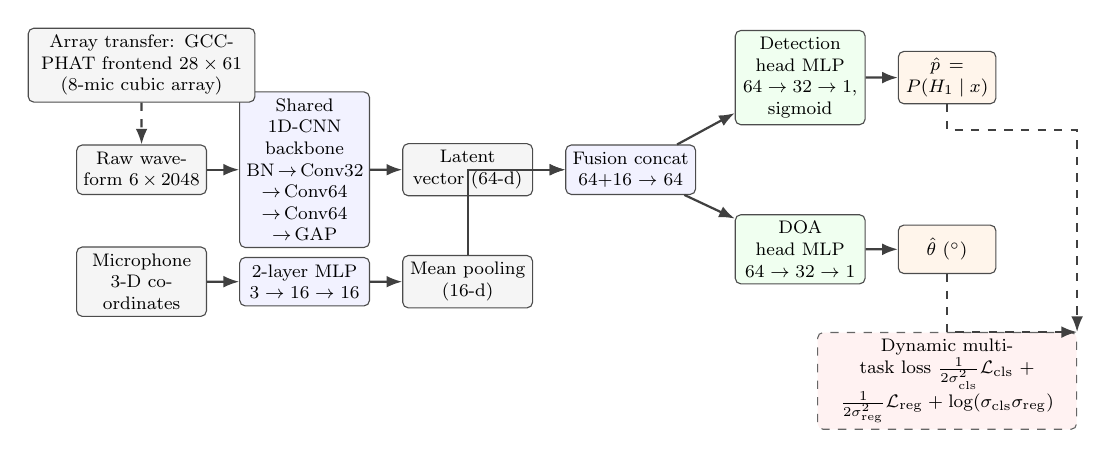
\begin{tikzpicture}[
    scale=0.82, transform shape, font=\footnotesize,
    node distance=4mm and 5mm,
    box/.style={rectangle, rounded corners=2pt, draw=black!70, fill=blue!5,
                align=center, inner sep=3pt, minimum height=7.5mm, text width=18mm},
    data/.style={box, fill=gray!8},
    head/.style={box, fill=green!6},
    outbox/.style={box, fill=orange!8, text width=13mm},
    loss/.style={rectangle, rounded corners=2pt, draw=black!60, dashed, fill=red!5,
                 align=center, inner sep=3pt, text width=38mm},
    arr/.style={-{Latex[length=2mm]}, thick, draw=black!75},
    darr/.style={arr, dashed},
]
% ---- signal path ----
\node[data] (in) {Raw waveform $6\times2048$};
\node[box, right=of in] (bb) {Shared 1D-CNN backbone\\ BN\,$\rightarrow$\,Conv32\\ $\rightarrow$\,Conv64\\ $\rightarrow$\,Conv64\\ $\rightarrow$\,GAP};
\node[data, right=of bb] (lat) {Latent vector (64-d)};
% ---- geometry path ----
\node[data, below=8mm of in] (mic) {Microphone 3-D coordinates};
\node[box, right=of mic] (mlp) {2-layer MLP $3\to16\to16$};
\node[data, right=of mlp] (pool) {Mean pooling (16-d)};
% ---- fusion ----
\node[box, right=of lat] (fuse) {Fusion concat $64{+}16\to64$};
% ---- heads and outputs ----
\node[head, above right=3mm and 6mm of fuse] (dh) {Detection head MLP $64\to32\to1$, sigmoid};
\node[head, below right=3mm and 6mm of fuse] (ah) {DOA head MLP $64\to32\to1$};
\node[outbox, right=of dh] (op) {$\hat p=P(H_1\mid\boldsymbol{x})$};
\node[outbox, right=of ah] (oa) {$\hat\theta$ ($^\circ$)};
% ---- loss ----
\node[loss, below=9mm of oa] (ls) {Dynamic multi-task loss $\frac{1}{2\sigma_{\mathrm{cls}}^{2}}\mathcal{L}_{\mathrm{cls}}+\frac{1}{2\sigma_{\mathrm{reg}}^{2}}\mathcal{L}_{\mathrm{reg}}+\log(\sigma_{\mathrm{cls}}\sigma_{\mathrm{reg}})$};
% ---- transfer annotation ----
\node[data, above=6.5mm of in, text width=33mm] (gcc) {Array transfer: GCC-PHAT frontend $28\times61$ (8-mic cubic array)};
% ---- arrows ----
\draw[arr] (in) -- (bb);
\draw[arr] (bb) -- (lat);
\draw[arr] (mic) -- (mlp);
\draw[arr] (mlp) -- (pool);
\draw[arr] (lat) -- (fuse);
\draw[arr] (pool) |- (fuse);
\draw[arr] (fuse) -- (dh);
\draw[arr] (fuse) -- (ah);
\draw[arr] (dh) -- (op);
\draw[arr] (ah) -- (oa);
\draw[darr] (op) |- ($(op.south)+(0,-4mm)$) -| (ls.north east);
\draw[darr] (oa) |- (ls.north east);
\draw[darr] (gcc) -- (in);
\end{tikzpicture}
\caption{Architecture of the proposed multi-task network. The two input branches are alternative front-ends for two array configurations: the raw multichannel waveform of the six-element ULA (top), and the geometry-aware GCC-PHAT feature map of the eight-element cubic array (bottom). The GCC-PHAT map has shape $28\times 61$ (28 microphone pairs $\times$ 61 correlation lags) and is fed to the shared 1D-CNN as a 28-channel one-dimensional signal of length 61, so the same backbone, detection head, and DOA head are reused across both front-ends; the 3-D microphone coordinates are encoded by a two-layer MLP, mean-pooled, and concatenated with the backbone features before the heads. Both heads are trained jointly under the uncertainty-based dynamic loss of~\eqref{eq:dynamic}, whose per-task log-variances are learned parameters.}
\label{fig:arch}
\end{figure}

\subsection{Shared 1D-CNN Backbone}
The raw $M\times N$ waveform is processed by a shared 1D-CNN that stacks temporal convolutions and pooling layers and flattens the result into a fixed-length latent vector used by both heads.

\subsection{Detection and DOA Heads}
Two lightweight heads branch from the latent vector:
\begin{itemize}
    \item a \emph{detection head} that outputs a scalar probability $p\in[0,1]$ (via sigmoid activation) for drone presence, trained using binary cross-entropy loss $\mathcal{L}_{\mathrm{cls}}$;
    \item a \emph{DOA head} that regresses the continuous azimuth $\hat\theta$, trained with an $\ell_1$ loss $\mathcal{L}_{\mathrm{reg}}$.
\end{itemize}

\begin{table}[H]
\centering
\caption{Configuration of the six-element ULA joint network (used for Table~\ref{tab:overall_compare}). K/S denotes kernel size/stride; zero-padding halves the temporal length each layer. The regression head uses an $\ell_1$ loss in degrees; the ground-truth azimuth is folded to $[0^\circ,180^\circ)$ (label $\theta\bmod 180^\circ$) and the test error uses the circular metric $\min\left(|\hat{\theta}-\theta|,\,180^\circ-|\hat{\theta}-\theta|\right)$. One forward pass over the $6\times2048$ input costs about $11.5$ M multiply-accumulate operations (roughly $22.9$ MFLOPs).}
\label{tab:net}
\small
\setlength{\tabcolsep}{4pt}
\begin{tabular}{llccc}
\toprule
Layer & Type & In$\rightarrow$Out & K/S & Params \\
\midrule
Input & -- & $6\times2048$ & -- & -- \\
BN & BN1d & $6$ & -- & $12$ \\
Conv1 & Conv1d & $6\to32$ & $5/2$ & $992$ \\
Conv2 & Conv1d & $32\to64$ & $5/2$ & $10\,304$ \\
Conv3 & Conv1d & $64\to64$ & $5/2$ & $20\,544$ \\
Pool & AvgPool1d & $64\to1$ & -- & $0$ \\
Det head & FC$\rightarrow$ReLU$\rightarrow$FC$\rightarrow$S & $64\to1$ & -- & $2\,113$ \\
Ang head & FC$\rightarrow$ReLU$\rightarrow$FC & $64\to1$ & -- & $2\,113$ \\
\midrule
\multicolumn{4}{r}{Total} & $36\,078$ \\
\bottomrule
\end{tabular}
\end{table}

\subsection{Dynamic Multi-Task Loss}
A common way to combine the two objectives is the fixed-weight form
\begin{equation}
    \mathcal{L}_{\mathrm{fix}} = \mathcal{L}_{\mathrm{cls}} + \lambda\,\mathcal{L}_{\mathrm{reg}},
    \label{eq:fixed}
\end{equation}
but a fixed $\lambda$ must be chosen by hand and trades detection against localization (Section~\ref{sec:results}). We therefore adopt the uncertainty-based balancing of Kendall \emph{et al.}~\cite{kendall2018mtl}, which learns this trade-off automatically, introducing one learnable scalar uncertainty $\sigma_k$ per task and minimizing
\begin{equation}
    \mathcal{L} = \frac{1}{2\sigma_{\mathrm{cls}}^{2}}\,\mathcal{L}_{\mathrm{cls}} + \frac{1}{2\sigma_{\mathrm{reg}}^{2}}\,\mathcal{L}_{\mathrm{reg}} + \log\!\left(\sigma_{\mathrm{cls}}\sigma_{\mathrm{reg}}\right).
    \label{eq:dynamic}
\end{equation}
Equation~\eqref{eq:dynamic} lends itself to a physical reading: $\sigma_{\mathrm{cls}}$ and $\sigma_{\mathrm{reg}}$ act as learnable ``observation noise'' levels for the classification and regression tasks, respectively---a task-wise homoscedastic uncertainty term---so that the precision factors $1/(2\sigma_k^{2})$ measure how reliable each task's residuals currently are. The gradient of~\eqref{eq:dynamic} with respect to the shared parameters $\mathbf{w}$ is
\begin{equation}
    \nabla_{\mathbf{w}}\mathcal{L} = \frac{1}{2\sigma_{\mathrm{cls}}^{2}}\,\nabla_{\mathbf{w}}\mathcal{L}_{\mathrm{cls}} + \frac{1}{2\sigma_{\mathrm{reg}}^{2}}\,\nabla_{\mathbf{w}}\mathcal{L}_{\mathrm{reg}},
    \label{eq:grad}
\end{equation}
so the effective convex weight on the classification gradient at training step $t$ is
\begin{equation}
    \lambda_t = \frac{\sigma_{\mathrm{reg}}^{2}(t)}{\sigma_{\mathrm{cls}}^{2}(t)+\sigma_{\mathrm{reg}}^{2}(t)}.
    \label{eq:lambda_t}
\end{equation}
Physically, $\lambda_t$ is the effective \emph{share} of the classification gradient in the combined parameter update: the complementary share $1-\lambda_t=\sigma_{\mathrm{cls}}^{2}(t)/(\sigma_{\mathrm{cls}}^{2}(t)+\sigma_{\mathrm{reg}}^{2}(t))$ is carried by the regression gradient. Monitoring $\lambda_t$ over training therefore gives a direct read-out of how the learned uncertainties trade the two tasks. In practice we optimize the log-variances $s_k=\log\sigma_k^{2}$ jointly with the network weights; this keeps $\sigma_k^{2}$ positive and the regularization term $\log(\sigma_{\mathrm{cls}}\sigma_{\mathrm{reg}})$ in~\eqref{eq:dynamic} prevents the trivial solution $\sigma_k^{2}\!\to\!\infty$. One caveat: the precision factor $1/(2\sigma_k^{2})$ can grow without bound if a task uncertainty collapses toward zero, risking instability; under our setup (log-variance parameterization, Adam $\eta=10^{-3}$, 20 epochs) training stayed stable with no clipping, but we recommend gradient clipping for noisier data or longer budgets. The ablation study in Section~\ref{sec:results} compares~\eqref{eq:dynamic} with the fixed-weight variants of~\eqref{eq:fixed} for $\lambda\in\{0.1,1.0,2.0\}$.

\subsection{Geometry-Aware Frontend for Array Transfer}
\label{sec:geo}
The raw-waveform backbone of Section~\ref{sec:method}-A is tied to the fixed six-element ULA geometry. To transfer the network to arrays with a different element count and layout, the variant used in Section~\ref{sec:real} replaces the raw input with a \emph{geometry-aware GCC-PHAT frontend}: for every microphone pair, the phase-transform cross-correlation~\cite{knapp1976gcc} is computed frame-wise and averaged, and a window of $61$ lags around zero delay is retained, yielding a $28\times61$ feature map for an eight-element array in which the azimuth information is concentrated in the correlation lag. In addition, the 3-D microphone coordinates are encoded by a two-layer perceptron; the resulting features are mean-pooled and concatenated with backbone features before being fed into the task heads, so that the heads are explicitly conditioned on the array geometry. The detection and DOA heads and the dynamic loss of~\eqref{eq:dynamic} are unchanged.

\section{Experimental Setup}
\label{sec:exp}
The simulation uses sampling rate $f_s=\SI{16}{\kilo\hertz}$, $M=6$ ULA elements, and an SNR sweep of $\{-10,-5,0,5,10,15\}\,\mathrm{dB}$. The training set comprises 4000 samples: $70\%$ drone-positive samples with the azimuth drawn uniformly from $[0^\circ,180^\circ)$ and $30\%$ pure-noise negative samples. A separate held-out validation set of 500 samples, generated by the same process with the same $30\%$ negative ratio and excluded from training, is reserved for detection-threshold selection, whereas all reported test metrics are computed on freshly generated Monte Carlo samples (600 per SNR) that are statistically independent of the training data. Negative samples are white Gaussian noise, and the channel noise added to positive samples is white Gaussian noise scaled to the prescribed SNR. Each training sample is assigned an SNR drawn uniformly at random from the six-level set $\{-10,-5,0,5,10,15\}\,\mathrm{dB}$ (equal probability), so a single model is exposed to the full range and is then evaluated across all SNRs without retraining. The network is trained with Adam ($\eta=10^{-3}$) for $20$ epochs with batch size $32$; the same trained model is evaluated at all SNR levels via Monte Carlo trials. The proposed network and the classical GCC-PHAT/SRP-PHAT baselines share the same synthetic signal model, array geometry, delay model and estimator code. The network entries of Table~\ref{tab:overall_compare} are taken from the per-SNR Monte Carlo protocol above (600 freshly drawn trials per SNR, statistically independent of the training data). The classical entries of the same table come from an \emph{independent} Monte Carlo draw that does not reuse the network test samples: it uses 60 trials whose SNR is drawn uniformly from the same six-level set instead of being pinned to $-5\,\mathrm{dB}$, and its detection operating point is taken from a separate 600-trial mixed-SNR energy-detector draw. The two families are therefore not paired on identical noise realizations, and no paired statistical test is claimed. The comparison nevertheless remains meaningful because the classical azimuth error is essentially independent of SNR (Fig.~\ref{fig:snr}), so a mixed-SNR mean lies within a fraction of a degree of any single-SNR value; the quoted $\pm$std and Monte Carlo standard errors are of comparable magnitude but derive from different draws. Baselines include the classical TDOA estimators GCC-PHAT~\cite{knapp1976gcc} and SRP-PHAT~\cite{dibiase2001srp}; learned DOA estimators (DOA-Net~\cite{adavanne2018doa}, SS-CNN~\cite{nguyen2020sscnn}, transformer~\cite{wang2024transformer,mack2022attention}) are discussed in related work but are not re-evaluated here. GCC-PHAT and SRP-PHAT are localization-only and have no intrinsic detector; for a fair comparison we equip them with a broadband energy test whose statistic is the total array energy $\sum_m\|x_m\|^2$ and whose threshold is the $95$th percentile of the noise-only energy, yielding an operating point near $P_{\mathrm{fa}}\approx0.05$. The classical baselines' $P_d/P_{\mathrm{fa}}$ quoted in Table~\ref{tab:overall_compare} are obtained from that same independent energy-detector draw (the broadband energy threshold is calibrated to the $95$th percentile of the noise-only energy), not from the $-5\,\mathrm{dB}$ anchor at which the network rows are reported; on a uniform linear array SRP-PHAT reduces to a GCC-PHAT-like delay-sum, which is why the two baselines give nearly identical MAE. We therefore focus our benchmark comparison on classical TDOA-based approaches and defer a head-to-head comparison with deep-learning DOA networks to future work; the reasons are that networks such as DOA-Net, SS-CNN, and transformer-based estimators consume phase spectra or spatial pseudo-spectra produced by a fixed frontend, whereas the present work regresses the azimuth directly from the raw multichannel waveform, so the input representation, model capacity, and computational budget differ across the two families and a head-to-head comparison would be unfair. All simulation results in this paper are fully reproducible from the accompanying code.\footnote{The main script \texttt{drone\_acoustic\_joint.py} regenerates all tables and figures in one run (\texttt{--mode sim}); it exports \texttt{data\_snr.csv} for Figure~\ref{fig:snr} and \texttt{table1\_repro.csv} for Table~\ref{tab:overall_compare}. The classical curves overlaid on Figure~\ref{fig:snr} are produced by \texttt{baseline\_snr.py}, which exports \texttt{baseline\_snr.csv}; it draws all randomness from locally seeded generators, so repeated runs give bit-identical output. Every script fixes its random seed before generating data or training, so the reported tables and curves are reproduced exactly. The code is released in a public repository at \url{https://github.com/wqinmin975/JointDetectionandAzimuthEstimation} and is also available from the corresponding author upon request during the review period.}

\subsection{Detection Threshold and Operating Point}
\label{sec:np}
Let $H_0$ denote the noise-only hypothesis and $H_1$ the drone-present hypothesis. The detection head outputs $p=\mathbb{P}(H_1\mid\boldsymbol{x})$, and a detection is declared when $p>\gamma$. The operating metrics are
\begin{equation}
    P_d(\gamma)=\mathbb{P}(p>\gamma\mid H_1), \qquad P_{\mathrm{fa}}(\gamma)=\mathbb{P}(p>\gamma\mid H_0),
    \label{eq:pdpfa}
\end{equation}
estimated over the Monte Carlo trials. On the held-out validation set of 500 samples we select, for each target false-alarm rate, the smallest threshold $\gamma^*$ that satisfies the Neyman--Pearson constraint $P_{\mathrm{fa}}(\gamma)\le P_{\mathrm{fa}}^{\mathrm{target}}$; sweeping $\gamma$ over $[0,1]$ yields the operating points reported below; because the detector is already near-saturated ($P_d\approx0.99$) at the minimum-error threshold in this synthetic regime, the resulting characteristic is near-degenerate, so we summarize it by the selected $\gamma^*$ operating points rather than plotting the full curve. For the target $P_{\mathrm{fa}}=0.01$, the selected threshold is $\gamma^*=0.086$ at every tested SNR from $-10$ to $15\,\mathrm{dB}$, giving a validation false-alarm rate of $0.0066$ and, at $\gamma^*$, a test-set detection probability of $1.00$ with a realized test false-alarm rate of $0.005$; relative to the default $\gamma=0.5$, the calibrated threshold also lifts the $-5\,\mathrm{dB}$ test detection probability from $0.99$ to $1.00$; these point estimates carry a Monte Carlo standard error of about $0.4\%$ (roughly 420 positive test samples at this SNR), so the two operating points are consistent within noise. Relaxing the target to $P_{\mathrm{fa}}=0.05$ lowers the threshold to $\gamma^*=0.038$ (validation $P_{\mathrm{fa}}=0.046$) and yields the same test detection probability of $1.00$ at a realized test false-alarm rate of $0.016$. The constancy of $\gamma^*$ across SNR reflects the large separation between the two hypothesis score distributions in this simulation: the constraint-optimal threshold is flat in SNR rather than rising as the SNR decreases, so a single threshold is adequate across the full tested range here. This convenience is a property of the synthetic data and should not be expected to transfer: under a harder regime, such as real non-stationary background noise, the Neyman--Pearson selection framework would need to be recalibrated, a direction flagged in the future work. Unless stated otherwise, all reported results use the default $\gamma=0.5$, the minimum-error decision under balanced priors, which satisfies the $1\%$ validation false-alarm constraint at every tested SNR (the validation false-alarm rate at $\gamma=0.5$ is $0.00$ at all SNR levels, i.e., zero false alarms on the $150$ negative validation samples).

\subsection{Metrics}
We report the detection probability $P_d$, the false-alarm rate $P_{\mathrm{fa}}$, and the DOA mean absolute error (MAE), with the CRB of~\eqref{eq:crb} as the theoretical lower bound on unbiased estimation error.

\subsection{Code Verification and Reproducibility}
\label{sec:repro}
The accompanying code reproduces every table and figure in one run (\texttt{--mode sim}); it exports \texttt{data\_snr.csv} (Fig.~\ref{fig:snr}) and \texttt{table1\_repro.csv} (Table~\ref{tab:overall_compare}). During development we identified and corrected a defect in the simulation's delay model: inter-microphone delays were computed but never applied to the individual channels, so the effective TDOA was zero and the synthetic data carried no azimuth-dependent acoustic cues. In the corrected model the 3-D source direction is projected onto the true array geometry; this corrected model is used for all experiments reported in this paper and the released code contains the corrected implementation, and no results obtained with the defective model are reported. As a sanity check, after the correction the trained network's azimuth MAE ($5.28^\circ$ at $\mathrm{SNR}=-5\,\mathrm{dB}$) is far below both the $90^\circ$ uniform-random baseline and the $\approx45^\circ$ folded-chance level of the classical GCC-PHAT/SRP-PHAT baselines (Table~\ref{tab:overall_compare}); this demonstrates that the corrected synthetic data carries the azimuth-dependent cues the network learns. The flat $\approx45^\circ$ classical baselines are a narrowband-PHAT artefact (Section~\ref{sec:results}), not a sign that the data lacks bearing information, and the CRB of $0.32^\circ$ (Table~\ref{tab:overall_compare}) independently confirms that the signal is highly informative.

\section{Results and Discussion}
\label{sec:results}
\subsection{Overall Performance Comparison}
Table~\ref{tab:overall_compare} reports the ablation variants and the CRB at $\mathrm{SNR}=-5\,\mathrm{dB}$, all reproduced by the accompanying code. The proposed dynamic scheme attains a detection probability of $0.99$ at a false-alarm rate of $0.00$ and an azimuth MAE of $5.28^\circ\pm5.57^\circ$, reducing the error of the classical GCC-PHAT and SRP-PHAT baselines ($45.24^\circ$ and $44.91^\circ$) by roughly a factor of eight. Joint training is essential: the detection-only branch learns no angle (MAE $46.38^\circ$) and the localization-only branch cannot discriminate drone presence from noise ($P_d=0.60$ at $P_{\mathrm{fa}}=1.00$). Among the multi-task variants the choice of loss weighting is a second-order factor: at $-5\,\mathrm{dB}$ the four settings all fall within a narrow $5.28^\circ$--$5.57^\circ$ band, with the fixed weights $\lambda=0.1$, $1.0$, and $2.0$ reaching $5.57^\circ\pm3.96^\circ$, $5.37^\circ\pm4.67^\circ$, and $5.46^\circ\pm4.90^\circ$ against $5.28^\circ\pm5.57^\circ$ for the dynamic scheme---spreads of the same order as the Monte Carlo standard error (about $0.27^\circ$ for roughly 420 positive test samples). The dynamic scheme anchors the low end of this band without any manual search, but the clear message of the ablation is that joint training, not the weighting scheme, drives the accuracy gain. The CRB of~\eqref{eq:crb} is evaluated for the same 2048-sample observation window as the network input, and the learned estimator remains above this bound at every SNR tested. We note that $\mathrm{CRB}(\theta)\propto1/\sin^2\theta$ diverges as $\theta\to0^\circ$ or $180^\circ$, so a full angular average of the CRB over $[0^\circ,180^\circ)$ is unbounded; we therefore report the conventional broadside reference $\theta=90^\circ$ rather than an average, while the network MAE is the corresponding average over the test azimuth distribution. The error saturation at about $3^\circ$ for $\mathrm{SNR}\ge5\,\mathrm{dB}$ is no longer noise-limited but reflects the finite capacity of the regression head together with the 2048-sample observation window and the 4000-sample training set. The remaining gap to the CRB ($0.32^\circ$ at $-5\,\mathrm{dB}$, and lower still at higher SNR) indicates that the learned estimator does not yet achieve efficient estimation; closing this gap would call for larger model capacity and more training data, which we leave to future work.

The comparison across SNR operating points reinforces this picture. At $-10\,\mathrm{dB}$ the dynamic scheme attains an azimuth MAE of $10.53^\circ\pm8.17^\circ$, versus $12.60^\circ\pm8.02^\circ$, $10.31^\circ\pm7.70^\circ$, and $10.98^\circ\pm7.94^\circ$ for the fixed weights $\lambda=0.1$, $1.0$, and $2.0$; at $0\,\mathrm{dB}$ the corresponding MAEs are $3.39^\circ\pm3.66^\circ$, $2.96^\circ\pm2.76^\circ$, $3.26^\circ\pm2.95^\circ$, and $3.27^\circ\pm3.10^\circ$. At $\mathrm{SNR}\ge-5\,\mathrm{dB}$ the four multi-task variants stay within $0.6^\circ$ of one another, whereas at $-10\,\mathrm{dB}$ the detection-biased $\lambda=0.1$ setting trades localization away and falls up to $2.3^\circ$ behind. The point-estimate winner among the fixed weights changes with the operating point ($\lambda=1.0$ at $-10\,\mathrm{dB}$, $\lambda=0.1$ at $0$--$10\,\mathrm{dB}$, $\lambda=2.0$ at $15\,\mathrm{dB}$, with the dynamic scheme lowest at $-5\,\mathrm{dB}$), so no single fixed weight is uniformly optimal without per-SNR re-tuning, while the dynamic scheme attains competitive accuracy at every tested SNR with no search at all. The two schemes also differ in robustness to the training budget: stretching it to $30$ epochs makes the fixed $\lambda=2.0$ variant overload, its $-5\,\mathrm{dB}$ MAE deteriorating from $5.46^\circ$ to $10.76^\circ$ and its $P_d$ from $0.988$ to $0.943$, whereas the dynamic scheme degrades more gracefully, from $5.28^\circ$ to $7.25^\circ$, with $P_d$ declining only from $0.991$ to $0.981$. All reported results therefore use the $20$-epoch budget.

\begin{table}[H]
\renewcommand{\arraystretch}{1.2}
\caption{Overall performance comparison of the classical TDOA baselines, ablation variants, and the proposed method, reproduced by the accompanying code. The network and ablation rows are reported at the $\text{SNR}=-5\,\text{dB}$ anchor; the two classical rows come from an independent Monte Carlo draw of 60 trials whose SNR is drawn uniformly from the same six-level set, with the detection operating point taken from a separate 600-trial mixed-SNR energy-detector draw (see Section~\ref{sec:repro}), so the classical entries are not paired sample-by-sample with the network entries. Because the classical azimuth error is nearly flat in SNR (Fig.~\ref{fig:snr}), the mixed-SNR classical mean is directly comparable to the $-5\,\text{dB}$ network value. The MAE column reports mean $\pm$ per-sample standard deviation over the Monte Carlo test set; $P_d$ and $P_{\mathrm{fa}}$ are point estimates from the same set. Fixed-weight variants follow $\mathcal{L}_{\mathrm{fix}}=\mathcal{L}_{\mathrm{cls}}+\lambda\mathcal{L}_{\mathrm{reg}}$ in~\eqref{eq:fixed}. The Cram\'er--Rao bound (CRB) at $\theta=90^\circ$ is provided as the theoretical lower bound. The proposed method is highlighted in bold. Learned DOA estimators (DOA-Net, SS-CNN, transformer) are discussed in related work but not re-evaluated here. All tabulated detection results use the default minimum-error threshold $\gamma=0.5$; a reported $P_{\mathrm{fa}}=0.00$ means zero false alarms among the 180 negative test samples at this SNR, whose upper 95\% confidence bound is about $1.7\%$.}
\label{tab:overall_compare}
\centering
\begin{tabular}{lccc}
\toprule
Method & $P_d$ & $P_{\mathrm{fa}}$ & Azimuth MAE ($^\circ$) \\
\midrule
\multicolumn{4}{l}{\textit{Classical TDOA Baselines}} \\
GCC-PHAT~\cite{knapp1976gcc} & $1.00$ & $0.05$ & $45.24\pm26.76$ \\
SRP-PHAT~\cite{dibiase2001srp} & $1.00$ & $0.05$ & $44.91\pm25.27$ \\
\midrule
\multicolumn{4}{l}{\textit{Ablation Variants (Multi-Task Analysis)}} \\
Detection-Only Branch & $1.00$ & $0.00$ & $46.38\pm26.07$ \\
Localization-Only Branch & $0.60$ & $1.00$ & $6.20\pm4.40$ \\
Fixed $\lambda=0.1$ (detection-biased) & $1.00$ & $0.00$ & $5.57\pm3.96$ \\
Fixed $\lambda=1.0$ (equal weight) & $0.995$ & $0.00$ & $5.37\pm4.67$ \\
Fixed $\lambda=2.0$ (localization-biased) & $0.988$ & $0.00$ & $5.46\pm4.90$ \\
\midrule
\multicolumn{4}{l}{\textit{Proposed Method and Theoretical Bound}} \\
\textbf{Proposed Dynamic Multi-Task Joint Model} & $\mathbf{0.99}$ & $\mathbf{0.00}$ & $\mathbf{5.28\pm5.57}$ \\
Cram\'er--Rao Lower Bound (CRB) & N/A & N/A & $0.32$ \\
\bottomrule
\end{tabular}
\end{table}

\subsection{SNR Sensitivity}
Fig.~\ref{fig:snr} plots $P_d$ and DOA MAE versus SNR from \texttt{data\_snr.csv}. The detection probability is near-saturated ($\ge0.985$) across the tested range and tends to improve with SNR; the proposed method's MAE lies above the CRB at every SNR. For reference, the classical GCC-PHAT and SRP-PHAT baselines remain near $45^\circ$ MAE and are essentially flat across the whole SNR range (Fig.~\ref{fig:snr}): their error is dominated by the narrowband tonal ambiguity and the ULA geometry rather than by noise, and on this six-element ULA SRP-PHAT reduces to a GCC-PHAT-like steered-response scan, so the two classical curves stay within a few degrees of one another and both stay in the $43^\circ$--$49^\circ$ band over the whole range. This is precisely the gap the learned joint model closes.

\begin{figure}[H]
\centering
\begin{subfigure}{0.48\linewidth}
\centering
\begin{tikzpicture}
\begin{axis}[
width=0.8\linewidth,
xlabel={SNR (dB)},
ylabel={$P_d$},
grid=major,
legend pos=south east,
ymin=0.98, ymax=1.005,
ytick={0.98,0.99,1.00},
yticklabel style={/pgf/number format/fixed, /pgf/number format/precision=3},
]
\addplot[mark=o,blue,thick] table [x=snr,y=pd,col sep=comma] {data_snr.csv};
\legend{Proposed};
\end{axis}
\end{tikzpicture}
\caption{Detection probability $P_d$ versus SNR.}
\end{subfigure}\hfill
\begin{subfigure}{0.48\linewidth}
\centering
\begin{tikzpicture}
\begin{axis}[
width=0.8\linewidth,
xlabel={SNR (dB)},
ylabel={DOA MAE ($^\circ$)},
grid=major,
legend pos=north east,
]
\addplot[mark=o,blue,thick] table [x=snr,y=mae,col sep=comma] {data_snr.csv};
\addplot[black,dashed,thick] table [x=snr,y=crb,col sep=comma] {data_snr.csv};
\addplot[red,thick] table [x=snr,y=gcc_mae,col sep=comma] {baseline_snr.csv};
\addplot[red,dashed,thick] table [x=snr,y=srp_mae,col sep=comma] {baseline_snr.csv};
\legend{Proposed,CRB,GCC-PHAT,SRP-PHAT};
\end{axis}
\end{tikzpicture}
\caption{Azimuth MAE versus SNR, with the Cram\'er--Rao bound (CRB) shown as the theoretical reference.}
\end{subfigure}
\caption{Detection probability $P_d$ and azimuth MAE versus SNR. Detection probability increases and azimuth MAE decreases as SNR rises; MAE saturates near $3^\circ$ at high SNR. The proposed method's error stays above the CRB across the full tested SNR range. Note that the vertical axis of subplot (a) starts from $0.98$ for better visualization of subtle detection-probability variations. The small non-monotonicity near $0\,\mathrm{dB}$ ($P_d\approx0.987$) is within the Monte Carlo standard error (about $0.4\%$ for 600 samples) and is not a meaningful trend. In subplot (b), the classical GCC-PHAT and SRP-PHAT baselines (evaluated by an independent Monte Carlo draw of 600 trials per SNR, see Section~\ref{sec:repro}) are nearly flat across the whole SNR range, staying in the $43^\circ$--$49^\circ$ band, and lie far above the proposed curve: their error is dominated by the narrowband tonal ambiguity and the ULA geometry rather than by noise, and on this six-element ULA SRP-PHAT collapses to a GCC-PHAT-like steered-response scan, so the two classical curves remain within a few degrees of each other. The learned joint model's SNR-dependent gain is therefore the decisive difference.}
\label{fig:snr}
\end{figure}

\subsection{Real-World Validation on Recorded Drone Audio}
\label{sec:real}
All results above are numerical simulations with the six-element ULA and the raw-waveform frontend of Sections~\ref{sec:signal}--\ref{sec:method}, and---consistent with the limitations noted in the Introduction---they assume an ideal array manifold (no element self-noise, gain mismatch, channel failure, or geometry calibration error). We now test transfer to real signals on two publicly available corpora: the Fraunhofer IDMT dataset, used to assess \emph{network} transfer of the learned model, and the Western Sydney University (WSU) corpus, used to assess the \emph{classical} baselines and, crucially, to obtain a real-world detection ROC that the IDMT set cannot provide (it lacks background-only negatives).

\subsubsection{Fraunhofer IDMT: network transfer to recorded audio}
\label{sec:real_idmt}
We first evaluate network transfer using the Fraunhofer IDMT real-world drone audio dataset~\cite{idmt2025drone}, recorded with the eight-element cubic microphone array also used for neural drone localization in~\cite{yang2025eusipco}; it contains 163 thirty-second segments of eight-channel audio at \SI{48}{\kilo\hertz} (PCM-16), and each segment ships with a GPS-derived ground-truth azimuth. The recordings capture several consumer UAVs (DJI Phantom 4, DJI Mavic, and Align models) in outdoor flight, whose acoustic signature is broadband rotor harmonics rather than the single \SI{800}{\hertz} tone of the simulator.

Because the cubic array is neither a ULA nor a six-element array, we replace the raw-waveform input with the geometry-aware GCC-PHAT frontend of Section~\ref{sec:geo}, which yields a $28\times 61$ feature map for the eight microphones. Concretely, each eight-channel segment is downsampled to \SI{16}{\kilo\hertz} and framed with a \SI{2048}{}-sample (\SI{128}{\milli\second}) Hann window and \SI{1024}{}-sample (\SI{64}{\milli\second}) hop; for every one of the 28 microphone pairs the GCC-PHAT correlation is computed frame-wise, averaged across frames, truncated to the central 61 lags, and max-normalized to peak 1. We distinguish the \SI{2048}{}-sample \emph{analysis frame} used by the GCC-PHAT frontend from the \SI{1.0}{\second} \emph{evaluation window} used for labeling and supervision: each \SI{30}{\second} segment is grouped into 30 non-overlapping evaluation windows (after downsampling), yielding $163\times30=4890$ windows; the per-window azimuth label is obtained by circularly interpolating the segment's GPS azimuth sequence and folding to $[0^\circ,180^\circ)$, and the fine-tuned model is supervised per window. The exact microphone positions of the IDMT cube are used both to compute the features and as the geometric conditioning input to the heads; the signal is downsampled to \SI{16}{\kilo\hertz} and a single global gain matches the real RMS level to that of the synthetic training input. The simulation's delay model was corrected before all experiments (see Section~\ref{sec:repro}); no results from the defective model are reported. The same multi-task backbone is trained on the corrected simulation and evaluated two ways: \emph{zero-shot} (simulation-trained weights unchanged) and \emph{fine-tuned} (continued training on all 163 real segments with Adam at a learning rate of $10^{-4}$ for $8$ epochs, using the per-window ground-truth azimuth as target). Because the corpus is small, no held-out split is made: the fine-tuned model is trained and evaluated on the same 163 segments, so the fine-tuned MAE of $18.1^\circ$ is an optimistic in-sample estimate rather than a generalization result, and evaluation on independently recorded flights is left to future work. A cubic array suffers from a front--back mirror ambiguity: a source and its mirror image about the array plane produce identical TDOAs, an inherent physical limitation of the array geometry rather than a deficiency of the algorithm. We therefore fold the azimuth into $[0^\circ,180^\circ)$ and report the error as circular error under the $180^\circ$\, periodicity.

Table~\ref{tab:real} and Fig.~\ref{fig:real} summarize the outcome. Zero-shot, the azimuth MAE is $45.6^\circ$\, with a correlation of $-0.21$ between prediction and folded ground truth: the broadband, real-world signature still lies outside the synthetic acoustic model, so the simulation-trained regressor does not transfer. After fine-tuning on the 163 real segments, however, the azimuth MAE drops to $\mathbf{18.1^\circ}$\, and the correlation rises to $\mathbf{+0.73}$, and the per-type breakdown shows consistent gains (Mavic $12.7^\circ$, Phantom4 $18.3^\circ$, Align $26.7^\circ$). This resolves the zero-shot failure: given real-world supervision, the localization branch adapts to real recordings once the frontend is geometry-aware and the simulation properly encodes time-delay information. The persistent zero-shot gap and the weaker Align-class error point to the broadband acoustic domain gap and to data scarcity as the open problems, not to a flawed architecture: the Align class shows the largest error ($26.7^\circ$) because it contributes the smallest number of recorded segments ($n=16$), and enlarging its recordings would allow a more reliable per-type assessment. As noted above, the fine-tuned figures are in-sample results---the model is evaluated on the same 163 segments used for adaptation---and should be read as an optimistic in-sample estimate, not a generalization result.

\paragraph{Detection note:}
The detection probability is $1.00$ in both settings, but this is of limited significance: the IDMT corpus contains only drone-present segments, so the false-alarm rate is undefined (no negative samples) and $P_d=1.00$ merely restates that every drone segment is flagged. The detection/false-alarm results of Table~\ref{tab:overall_compare} therefore rest entirely on the synthetic study; a meaningful real false-alarm study requires background-only negatives, which we supply via the WSU corpus in Section~\ref{sec:real_wsu}.

\paragraph{Setup assumptions:}
Two pipeline assumptions warrant stating. First, the eight WAV channels are assumed to map one-to-one to the eight microphones per the IDMT geometry; a channel permutation would rotate the reconstructed array and bias every estimate, so empirical calibration of this mapping is advisable before field deployment. Second, the IDMT ground truth stores elevation as a zenith angle ($90^\circ$ = horizontal plane) and the flights are near-horizontal, so we report azimuth only and leave elevation estimation to future work.

\begin{table}[H]
\renewcommand{\arraystretch}{1.2}
\caption{Real-world validation on the Fraunhofer IDMT dataset~\cite{idmt2025drone} (163 segments, eight-element cubic array). The simulated row is the proposed model at $\mathrm{SNR}=-5\,\mathrm{dB}$ from Table~\ref{tab:overall_compare}. Zero-shot uses the simulation-trained weights (GCC-PHAT frontend, corrected delay model) unchanged; fine-tuned continues training on all 163 real segments with per-window azimuth supervision. Azimuth MAE is reported under the $180^\circ$ circular fold. Fine-tuned results are obtained by training and evaluating on the same 163 segments, representing an optimistic in-sample estimate, not a generalization result.}
\label{tab:real}
\centering
\setlength{\tabcolsep}{4pt}
\begin{tabular}{p{0.46\linewidth}p{0.27\linewidth}p{0.18\linewidth}}
\toprule
Setting & Detection Probability $P_d$ & Azimuth MAE ($^\circ$) \\
\midrule
Simulation (proposed, $-5\,\mathrm{dB}$) & $0.99$ & $5.28\pm5.57$ \\
Real audio, zero-shot (GCC-PHAT, corrected simulation) & $1.00$ & $45.55\pm16.78$ \\
Real audio, fine-tuned (163 segments) & $1.00$ & $\mathbf{18.05\pm12.75}$ \\
\bottomrule
\end{tabular}
\end{table}

\begin{figure}[H]
\centering
\includegraphics[width=\linewidth]{real_eval.png}
\caption{Real-world validation on the Fraunhofer IDMT dataset. (Left) Zero-shot predicted versus ground-truth azimuth (folded to $[0^\circ,180^\circ)$): predictions scatter far from the diagonal, showing the simulation-to-reality acoustic gap. (Center) Fine-tuned predicted versus ground-truth azimuth: points concentrate near the diagonal, confirming that the localization branch transfers once the frontend is geometry-aware and the simulation encodes the true delays. (Right) Per-type azimuth MAE for zero-shot and fine-tuned: fine-tuning lowers the error for every drone class.}
\label{fig:real}
\end{figure}

\subsubsection{Western Sydney University corpus: classical baselines and detection}
\label{sec:real_wsu}
Because the IDMT corpus lacks background-only negatives, we evaluate the classical GCC-PHAT/SRP-PHAT baselines on the Western Sydney University (WSU) UAV Acoustic Localization Dataset~\cite{wsu2024dataset} to obtain a real-world ROC. WSU records DJI Air~3 flights on a calibrated 24-element 3-D array (four Zoom F6 recorders, \SI{48}{\kHz}, \SI{32}{bit} integer WAV) with GPS-synced azimuth. We use two sessions: \textbf{test1} (\texttt{Oct\_11\_2024/flight\_5}, an unseen quiet site, \num{1592} drone frames) and \textbf{test2} (\texttt{Mar\_18\_2025/flight\_2}, loud wind/traffic, \num{11927} drone frames plus a labeled background-only tail, seconds 1577--1864, \num{2871} frames). Signals are band-limited to \SI{200}{}--\SI{4000}{\Hz} and framed at \SI{0.1}{\s}; GPS rows are aligned to frames by nearest index. Ground-truth azimuth is reproduced in a local ENU frame (the UTM offset cancels), with a per-session north-alignment offset from \texttt{initial\_azimuth\_deg}. For each of the $\binom{24}{2}=276$ pairs we take the PHAT peak lag as the TDOA and fuse by least squares ($\mathbf{M}\mathbf{d}=c\boldsymbol{\tau}$, no robust rejection); SRP-PHAT grid-searches azimuth$\times$elevation over $[0^\circ,360^\circ)\times[0^\circ,60^\circ]$ ($2^\circ\times4^\circ$), taking the peak steered response. Detection uses frame energy and the SRP-power peak, with ROC/AUC from 200 thresholds (drone frames positive, \texttt{no\_drone} negative).

Table~\ref{tab:wsu_mae} reports the azimuth MAE folded to $[0^\circ,180^\circ)$ (the IDMT convention). For a uniform-random estimate the expected folded error is exactly $45^\circ$, so $\approx45^\circ$ means the \emph{chance level} of this metric, not a resolved bearing. On real data GCC-PHAT reaches $44.5^\circ$--$45.4^\circ$ and SRP-PHAT $37.5^\circ$ (test1) to $45.4^\circ$ (test2)---consistent with, not a reproduction of, the flat synthetic baseline of Section~\ref{sec:results} ($\approx45^\circ$ GCC-PHAT and $\approx44.9^\circ$ SRP-PHAT, flat from $-10$ to $+15$ dB SNR).

The flatness is \emph{not} a spatial-aliasing effect. The synthetic rotor signature is an \SI{800}{\hertz} carrier amplitude-modulated at \SI{120}{\hertz} (Section~\ref{sec:signal}), well below the ULA spatial Nyquist $c/(2d)\approx\SI{2.14}{\kHz}$, so no grating lobe is present. Instead, PHAT whitens every frequency bin by its magnitude, so a narrowband tone occupying only a few bins leaves thousands of noise-dominated bins with equal weight; the whitened cross-spectrum is therefore dominated by noise and the GCC-PHAT/SRP-PHAT estimates become SNR-independent, collapsing to the $\approx45^\circ$ folded-chance level exactly as observed across all SNRs. On the real \num{24}-element array the same $\approx45^\circ$ for GCC-PHAT reflects fragile least-squares TDOA fusion without outlier rejection, whereas SRP-PHAT's grid search is more robust---why SRP-PHAT beats GCC-PHAT on real data while the two coincide under the noise-free synthetic model.
\begin{table}[H]
\centering
\caption{Classical azimuth MAE ($^\circ$, folded to $[0^\circ,180^\circ)$) on WSU field recordings. The folded metric has a chance level of $45^\circ$.}
\label{tab:wsu_mae}
\begin{tabular}{lccc}
\toprule
Session & $N_{\text{drone}}$ & GCC-PHAT MAE ($^\circ$) & SRP-PHAT MAE ($^\circ$) \\
\midrule
test1 (quiet) & \num{1592} & $44.51\pm25.87$ & $37.46\pm27.99$ \\
test2 (loud) & \num{11927} & $45.37\pm26.06$ & $45.39\pm24.82$ \\
\bottomrule
\end{tabular}
\end{table}

Folding conceals the front-back ($180^\circ$) ambiguity inherent to a low-elevation source: on test1, 17\% (GCC-PHAT) and 38\% (SRP-PHAT) of frames are flipped, driving the unfolded error to $89^\circ$/$105^\circ$ vs.\ the folded $45^\circ$/$37.5^\circ$; the IDMT evaluation shares this mirror defect.

Table~\ref{tab:wsu_roc} and Fig.~\ref{fig:wsu} give the detection ROC. Energy retains some discrimination on quiet test1 ($AUC=0.67$) but degrades to $AUC=0.50$ (random) on loud test2; the SRP-power statistic stays near chance ($AUC\le0.53$ everywhere). test1 contributes only \num{54} background-only frames (a short ambient tail within the same \texttt{Oct\_11\_2024/flight\_5} session), so its $AUC=0.67$ carries a wide 95\% CI ($\pm0.12$); test2's \num{2871} negatives, by contrast, come from a dedicated labeled background-only recording (seconds 1577--1864). The implication is direct: simple energy/spatial-coherence detectors are unreliable under loud ambient noise, motivating the learned detector and the Neyman--Pearson operating point of Section~\ref{sec:np}; the present result---classical detection collapses as ambient grows, and $\gamma^*$'s constancy cannot be relied upon off the synthetic set---is the empirical confirmation of that section's warning.
\begin{table}[H]
\centering
\caption{ROC AUC of classical detectors on WSU: drone frames versus background-only segments. SRP-power remains near chance ($AUC\le0.53$) in every subset.}
\label{tab:wsu_roc}
\begin{tabular}{lcccc}
\toprule
Subset & $N_{\text{drone}}$ & $N_{\text{amb}}$ & Energy AUC & SRP-power AUC \\
\midrule
Combined & \num{13519} & \num{2925} & 0.500 & 0.492 \\
test1 (quiet) & \num{1592} & \num{54} & 0.669 & 0.528 \\
test2 (loud) & \num{11927} & \num{2871} & 0.500 & 0.505 \\
\bottomrule
\end{tabular}
\end{table}
\begin{figure}[H]
\centering
\includegraphics[width=\linewidth]{wsu_roc.png}
\caption{Classical baselines on the WSU real-world corpus. (Left) ROC for energy-based (solid) and SRP-power (dashed) detectors per subset and combined; the diagonal is chance. (Right) folded azimuth MAE of GCC-PHAT and SRP-PHAT on WSU, versus the synthetic baseline ($\approx45^\circ$, Section~\ref{sec:results}).}
\label{fig:wsu}
\end{figure}

Scope: the learned network is \emph{not} evaluated on WSU (different array geometry, no domain adaptation here); the WSU results concern the classical baselines only. The corpus has a single UAV model, and is an ideal future test-bed for the network via the geometry-aware frontend of Section~\ref{sec:geo}.

\section{Conclusion}
\label{sec:conclusion}
This paper presented an end-to-end multi-task network that performs drone detection and azimuth estimation jointly from the raw multichannel waveforms of a six-element MEMS microphone array, replacing the conventional decoupled detection--localization pipeline. The joint design is preferable to a decoupled pipeline for two reasons: sharing one 1D-CNN backbone lets the two tasks exploit a common representation and prevents detection errors from propagating into the localization branch, and the uncertainty-based dynamic weighting of~\eqref{eq:dynamic} balances the classification and regression gradients during training without manual $\lambda$ tuning, sparing the cost of a loss-weight search. Monte Carlo simulations show that the joint model detects the drone with $P_d\approx0.99$ at $P_{\mathrm{fa}}\approx0$ and localizes it at $5.3^\circ$ azimuth MAE at $\mathrm{SNR}=-5\,\mathrm{dB}$, cutting the error of the classical GCC-PHAT and SRP-PHAT baselines by roughly a factor of eight. The ablation study confirms that joint training is necessary: a detection-only branch learns no angle, while a localization-only branch yields no usable detection decision ($P_d=0.60$ at $P_{\mathrm{fa}}=1.00$). The dynamic weighting attains accuracy competitive with the best tuned fixed weight at every tested SNR without any manual search, and degrades more gracefully when the training budget is extended.

The real-world test of Section~\ref{sec:real} shows that, once the input is replaced by a geometry-aware GCC-PHAT frontend on the true eight-element cubic array and the simulation's delay model is corrected, the joint multi-task backbone transfers to recorded drone audio: fine-tuning on the 163 real segments reduces the azimuth MAE from $45.6^\circ$ (zero-shot) to $18.1^\circ$ with a prediction--ground-truth correlation of $+0.73$. The WSU corpus (Section~\ref{sec:real_wsu}) supplies the background-only negatives the IDMT set lacks and shows that the classical GCC-PHAT/SRP-PHAT baselines remain at the folded-azimuth chance level on real field data while classical energy/spatial-coherence detection is near chance under loud ambient noise, directly motivating the learned detector and its Neyman--Pearson operating point. Several limitations remain. The simulation-to-reality acoustic gap is substantial---the $45.6^\circ$ zero-shot error shows direct transfer fails---and narrowing it calls for more realistic rotor-noise synthesis. Because the corpus is small, fine-tuning is performed and evaluated on the same 163 segments, so $18.1^\circ$ is an optimistic in-sample estimate and generalization to independent flights is unverified; moreover the IDMT corpus contains only drone-present audio, so real-signal false-alarm performance stays unvalidated. The method addresses a single source on an ideal array and does not model MEMS impairments (element self-noise, sensitivity mismatch, channel failures, geometry calibration error).

Future work will extend the model to multiple concurrent sources and to elevation estimation (which the cubic geometry supports), enlarge the real corpus with background-only negatives for a rigorous real false-alarm evaluation, synthesize more realistic rotor noise to narrow the domain gap, and---on the engineering side---improve robustness to channel gain mismatch, channel failure, and geometry calibration error while adapting the detection threshold to non-stationary noise and assessing embedded MEMS deployment and inference speed.


%=================================================================
\supplementary{The reproducibility package containing the simulation code, the exported result tables, and the rendered validation figures is provided as supplementary material; the accompanying LaTeX source of this manuscript and the MDPI class files are included in the same package.}

\authorcontributions{Conceptualization, Q.W. and L.T.; methodology, Q.W. and L.T.; software, Q.W.; validation, Q.W., Z.W., Z.H., H.W. and L.T.; formal analysis, Q.W.; investigation, Q.W.; resources, L.T.; data curation, Q.W.; writing---original draft preparation, Q.W.; writing---review and editing, Z.W., Z.H., H.W. and L.T.; visualization, Q.W.; supervision, L.T.; project administration, L.T.; funding acquisition, L.T. All authors have read and agreed to the published version of the manuscript.}

\funding{This research was funded by the National Natural Science Foundation of China under Grant No. 62101076, and by the 2025 Science and Technology Innovation Capability Enhancement Project of Guangdong University of Science and Technology under Grant No. GKY-2025BSQDK-46.}

\institutionalreview{Not applicable. This study is a numerical simulation combined with the evaluation of two publicly available, peer-reviewed acoustic corpora; it involved no human participants, no identifiable personal data, and no animal experiments.}

\informedconsent{Not applicable. This study involved no human participants; the two recorded drone-audio corpora used for validation are publicly available and contain no personally identifiable information.}

\dataavailability{The synthetic dataset and the accompanying simulation code are released by the authors. The recorded-drone corpora used for validation are publicly available: the Fraunhofer IDMT drone-audio dataset \cite{idmt2025drone} and the Western Sydney University UAV Acoustic Localization Dataset \cite{wsu2024dataset}.}

\acknowledgments{The authors acknowledge the support of the National Natural Science Foundation of China and Guangdong University of Science and Technology.}

\conflictsofinterest{The authors declare no conflicts of interest.}

%=================================================================
% References section title (the MDPI class leaves \@reftitle empty by default)
\reftitle{References}

\externalbibliography{yes}
\bibliography{refs}

%=================================================================
% Author biographies. The MDPI class provides the \bio command for this block
% (Definitions/mdpi.cls: \newcommand{\bio}[2]); it sets the author name in a
% narrow left column with the biography text in a 9pt pbox beside it, which is the
% MDPI house format. The block is placed after the References.
\section*{Author Biographies}

\bio{Liwei Tian}{received his M.Sc. degree from Guangxi Normal University, Guilin, China, in 2009, and his Ph.D. degree from Macau University of Science and Technology, Macau, China, in 2019. He is currently a Professor with the School of Computer and Artificial Intelligence, Guangdong University of Science and Technology, Dongguan, China. He is a Senior Member of the China Computer Federation (CCF) and a member of its Dongguan Branch Executive Committee, a member of the Technical Committee on Intelligent Simulation, Optimization and Scheduling of the Chinese Society of Simulation, and a member of the Technical Committee on Discrete and Intelligent Computing of the Chinese Association of Artificial Intelligence. His research interests include array signal processing, acoustic source localization, and multi-task deep learning for UAV detection and localization.}

\end{document}
